%If lack of simulation realism was one of the largest deterrents to adopting FireSim,
%modeling rationally related clocks is a stepping stone to building systems
%with dynamically scaling ones.  Useful for doing performance modeling.

Until now all Golden Gate and MIDAS-generated simulators modeled systems with a
single clock domain. Anecdotally, the lack of support for simulating targets
with more than a single clock has been the most common criticism of FireSim
offered by potential users FireSim, many of whom turn to using a conventional
FPGA prototype. The criticism is well justified. Most notably, forcing the outer memory
hierarchy to run at the speed of the cores results in a memory hierarchy that
can sustain artificially high bandwidths at lower latencies.

To date, the only effort to validate FireSim performance against a silicon
implementation was conducted Lee and Waterman~\cite{VLSIFireSimEval}, where they
compared SPECInt2006 results collected from the HiFive Unleashed~\cite{HiFiveUnleashed}
against an equivalent design running on FireSim. While the geomean of FireSim's
SPEC score fell within 2\% of the HiFive Unleashed, the largest difference was
10.7\% for \texttt{429.mcf}, a benchmark with infamously poor memory locality
(its working set has been measured 680 MB\cite{SPEC2006WorkingSet}). The
FireSim variant differed in that it used non-standard UC Berkeley IO devices
(and backing FireSim Bridges) and a FASED memory timing model instead of their
commerical DDR3/4 memory controller. Most notably, the HiFive Unleashed
coreplex and memory hierarchy spans three clock domains. Tiles run at the fastest
frequency~(1.5 GHz in their study), the uncore runs at half this frequency~(75O
MHz), and the DRAM memory system, capable of 2400 MT/s (resulting in a 600 MHz
controller clock in their implementation), sits in it's own clock domain behind
an asynchronous crossing\cite{FreedomU540}. In this case, if support for modeling
multiple clocks with fixed frequencies were supported in FireSim, bridges would
be the only remaining non-trivial source of simulation error in systems that do not
dynamically scale their frequencies.

A natural place to look for inspiration is in FPGA prototyping. Here,
supporting multiple clock domains is a relatively straightforward process in
theory. When mapping the ASIC design to the FPGA, clock generating circuits,
like a PLL, are replaced with FPGA equivalents~\cite{FPMM}. While the absolute
frequencies used in the prototype will be considerably slower due to frequency
limitations of the FPGA, the relative frequencies can be maintained, and thus
latencies through an SoC cache hierarchy can be properly modeled~(the
aforementioned problem of modeling off-chip memory systems like DRAM remains).
In practise, limited availability of clocking resources and restrictions in
FPGA clock distribution can sometimes require non-trivial changes to the ASIC
RTL. To ameliorate these challenges \emph{FPGA-Based Prototyping Methodology
Manual}~\cite{FPMM} suggests a number of Design-For-Prototyping techniques
including implementing only a subset of the clocking structures, sticking to
conventional synchronous design techniques, and isolating clock generation and
distribution structures in seperate modules at the top-level of the design
hierarchy.

% DVFS stuff, prototypes
Applying the prototyping approach to a decoupled simulator --- generating
multiple host-clocks whose relative frequencies match that of the target --- is
an abstraction breaking change conflates host and target concerns.  In practise
optimized models and bridges are going to be resident in different clock
domains, and thus it will be necessary to independently gate the different
host clocks, destroying much of the merit of generating multiple clocks in
the first place. Instead, multiple simulated clocks can be derived from a single
host clock. This approach has some appealing implications:
\begin{itemize}
 \item It does not require FPGA-specific clocking resources beyond clock
 buffers capable of gating the host clock. For smaller units where the fanout
 on the clock enable is small, even these can be avoided by directly adding a clock enable
 to all state elements instead of directly gating the clock. This makes it easier
 to port the same simulator to a different FPGA host.

 \item It simplies the implementation, since all simulator control logic is synchronous to 
 the same clock.
\end{itemize}

One potential benefit of generating host clocks with different frequencies is
that it has the potential to improve simulator throughput (\ref{eq:sim-perf})
by putting faster parts of the target in faster host clock domains (thus
improving the $f_{fpga}$ term). Intuitively, one would expect that a faster target clock
domain should close timing at higher frequency than a
slower one -- while this is generally true, the ratio of crtical-path delays
between clock domains can differ substantially from an ASIC implementation, most notably because delay through ASIC elements do
not scale uniformly across all structures when mapped to an FPGA~\cite{FPGAGap2}.
We do not rule out using multiple host-clocks in the future, rather, we
argue that host clock frequencies should be selected based on simulator
critical paths specifically to improve simulator throughput -- not as a means to enable
simulation of multiple clocks in the target.

Using a single host clock still enables a variety of implementation
styles. Our intial prototypes revolved around modeling clock-domain crossings
in channels. For example, one could model a two-to-one crossing from a fast clock
domain to a slow clock domain by dropping every second token or, if in the
reverse direction, duplicating every token once. An early prototype of this
approach can be found in FireSim version 1.4, which permitted users to
model a clock division in the crossing between the hub and an endpoint.
\TODO{Jenny} used thus to simulate a system with a DRAM memory systems running
at one third the rate of the rest of the simulator. To apply this technique across
the target and not simply between bridges, we considered using Golden
Gate's hierarchy manipulations to divide the target design into synchronous
islands. Each of these islands would become seperate units transformed with an unmodified FAME transform.
Then, in simulation mapping Golden Gate would synthesize wire-type CDC channels between
these islands\footnote{Note that the clock-domain crossing present in target still
exists, but it is split into two synchronous halves across the models. In the future, we could
pull these crossing-halves into the channel itself to improve simulation
performance.} Clock frequency information would be baked into
these clock-crossing channels during channel synthesis. We began a prototype implementation of this
approach~(we sketched out FIRRTL transformations to perform this partitioning
and designed the channels) before reconsidering.  This approach introduced
considerable structural changes to the design's module hierarchy, making the
simulator more difficult to debug, and complicating a reimplementation of
Strober-style state snapshotting. Secondly, it introduced non-trivial
amounts of queueing when cuts between clock domains spanned large sets of signals.
Perhaps most importantly, it was considerably more complex than the solution we
ultimately selected.

% Other systems that model multiple target clocks / related work.
% DVFS stuff, prototypes

% Other approaches we considered that are LI-BDN complaint
%- Doing stuff in thechannels, and splitting the design.
%  - Diagram?
%  - Used to model memory controllers in early versions of MIDAS.
%  - Ad-hoc, difficult to validate.

\section{Implementation}
% relation to ITDC / ETDC simulators

Our approach instead was to modify the hub unit to simulate multiple clock
domains \emph{in situ}. The hub unit instantiates seperate clock buffers for
each clock domain, and selectively fires clocks and channels based on the set
of clock edges it is scheduled to simulate. A single \emph{clock bridge},
generates the clock schedule as a token stream of bit-vectors indicating which
clocks are scheduled to fire in a given simulator timestep. For simplicity, we
mandate all other units, bridges and optimized models, continue to be
synchronous to a single clock. As a result, the resulting simulator remains
implicitly timestamped.

All other aforementioned restrictions on target RTL still apply. Aside from
the singleton clock bridge there must be no other clock generators in the
design. Specifically, when in FIRRTL's low form, all clock-type members of FIRRTL statements and expressions
must be driven by the clock bridge exclusively through a sequence of
\texttt{Connect} statements. Asynchronous resets are still coerced by the
compiler to synchronous ones.

Strictly speaking, a target with more than one clock cannot be an SSM. TODO{In
section}, we explain how multiclock RTL can be treated as an SSM under the
assumptions of our implementation, and discuss the implications of this
vis-a-vis verifying existing models.

\subsection{Annotation Modifications}

Where previously all channels were implicitly synchronous to the sole target
clock, now channels bound for different units may be synchronous to different
clocks. To support this, we extended channel annotations to carry a reference
to a clock in the hub model, so that the FAME transform may associate the
correct subset of channels with each clock domain. Bridge-emitted channel
annotations indicate their clock at instantiation time,
whereas compiler-extracted models have their clock inferred (more on this
later). Additionally, we introduced a new clock-type channel
field~(\texttt{TargetClockChannel}) to label the singleton clock channel in the
simulator as this channel must be handled specially by the FAME transform and channel
synthesis.

\subsection{Modified FAME Transform}
The bulk of the complexity in supporting multiple clock domains is contained in
modified FAME transform. We show the resulting hub unit implementation in
Figure~\ref{fig:static-multiclock-wrapper}. Unlike in the single-clock
implementation, the wrapper circuit must selectively operate on a subset of
channels based which clocks are scheduled to fire.  Output state machines (shown in
blue) remain mostly unchanged but are now selectively reset based on the
scheduled clock.  We added input FSMs (shown in green) to remove the fanout from
the clock token port to input channel dequeue. These too are selectively reset.

Clock scheduling is managed by a two-cycle control path (shown in orange). In
stage 1, input FSMs (in green) are reset; which allows them to dequeue an input
token in the execution of the second stage. In stage two, output FSMs are reset and a
pulse is through the target clock by enabling a dedicated clock buffer for that
domain. The pipeline advances under the largely the same firing condition as the
synchronous wrapper: all channel inputs are valid, including the clock channel, and all outputs have
enqueued or are enqueueing. Since output channels for clock domains not scheduled to fire in
stage two are not reset, their \texttt{fired} registers remain set and cannot stall the pipeline.
\TODO{handle clock token valid in diagram}

\begin{figure}
    \centering
    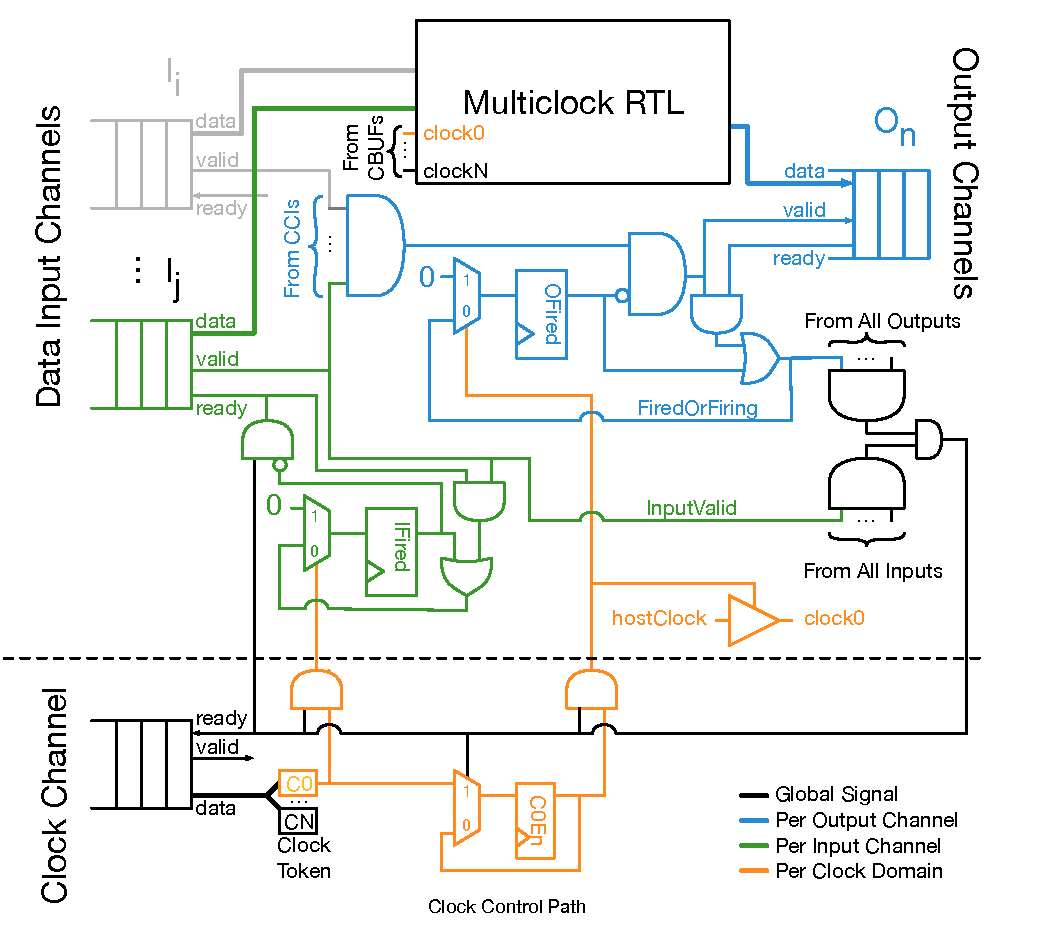
\includegraphics[width=0.99\textwidth]{figures/static-multiclock-wrapper.pdf}
    % graffle2pdf -c multiclock-wrapper midas-graphics/graffle/wrapper-transforms.graffle figures/static-multiclock-wrapper.pdf
    \caption{A wrapper-module-based conversion of multiclock target RTL with multiple clocks into a unit}
    \label{fig:static-multiclock-wrapper}
\end{figure}

\TODO{Is the extra register stage necessary?}

Initially all output FSMs are reset to zero, and the clock pipeline
register marked invalid (no clock is scheduled to fire).  This permits all combinational paths across all clock domains resolve based on the
initial input token values and target state.  As previously discussed, all
target clocks are gated under host reset such that BRAM and register state
initialized during FPGA programming cannot spuriously change as the FPGA comes
out of reset.

\subsection{Clock Bridge}

The clock bridge is responsible for determining the clock schedule by
generating an infinite token stream of $N$-wide bitvectors, where $N$ is the
number of clock domains in the target. Each clock token corresponds to a
simulator timestep. Any clock scheduled to fire in a given timestep will have
its bit set in the corresponding clock token.

The provided clock bridge implementation accepts clock specification that
defines the frequency of all clocks as rational multiple of the
frequency of the zeroth clock\footnote{Another reasonable approach would be to
specify the periods of all clocks in an agreed upon timebase. We note
that in this case all clocks are rationally related to a fast clock whose
period equals the resolution of the timebase.}. To model a clock that is not
rationally related (e.g., a periphery clock that generated by a
secondary PLL or is sourced from off-chip), the user should select a rational
multiple that would best match the desired frequency of the clock.  During
elaboration, the clock bridge determines a virtual fast clock from which all
output clocks can be derived via an integer division (in other words, it finds
a clocks whose frequency is the least common multiple of the frequency of the
requested clocks). Then, for each output clock, it generates a series of
down-counters (\texttt{timeToNextEdge}) which are systematically reset to the
division required to generate that output clock.

To generate an output token, the bridge does the min-reduction across
\texttt{timeToNextEdge}, and broadcasts the result. All outputs whose
\texttt{timeToNextEdge} matches the minimum are scheduled clocks: their bit is
set in the output token, and their \texttt{timeToNextEdge} register is reset to
their division. Unscheduled clocks subtract the broadcasted time delta from
their registers, simulating the advance of time.  This implementation is
capable of producing a clock token with at least one bit set every host cycle.

\subsection{Other Compiler \& Bridge Modifications}

In our and our users' experience, bridges are difficult to write as they force
the developer to reason about both host and target-time considerations. To
prevent further exacerbating this problem, we elected to forbid bridges and
extracted models from having channels in multiple clock domains. This had three
primary implications:

\begin{enumerate}
\item User-instantiated bridges must explicitly indicate the clock to which
they are synchronous. Bridge-emitted channel annotations contain references to
this clock. This is a relatively trivial change, but one that affects user
facing code.

\item Debug synthesis passes must emit multiple bridges. For example, assertion
synthesis must generate a new bridge for each clock domain in which there is at
least one assertion. To do so, we built FIRRTL analyses to find source clocks
        by walking clock connectivity~(\texttt{FindClockSources}), and to group and wire
nodes (like an assertion condition) to the top-level based on each nodes source
clock(~\texttt{BridgeTopWiring}).

\item To populate channels with references to clocks in extracted models, we
introduced a transform (\texttt{FindDefaultClocks}, run before \texttt{ChannelExcision}) that analyzes top-level
clock connectivity between extracted models and the hub. Any stateful module
once extracted will have connection between a new clock output port on the hub
module and a sink port on the model (the latter port was extant prior to extraction). By
finding these connections, models can be labelled with a clock reference on the
hub model and their channels anontations can be subsequently updated.
\end{enumerate}

\subsection{The Base Clock}

One consequence of simulating systems with a single global clock is that it is
natural to specify time in cycles of that clock. Bridges can trivially track
time with a counter that tracks the number of times it has fired. Introducing
multiple clocks complicates this: specifications of time must either be made
explicit, or specified in clock cycles of some agreed upon common clock. In
either case, these specified times cannot be compared against a bridge-local
cycle counter without the local clock's frequency, or its relative frequency to
the agreed-upon common clock. Many of FireSim's features use specifications of global time. For example,
instrumentation bridges (like tracerV, assertion, and print bridges) accept
runtime arguments that specify windows of time overwhich they should be
enabled. Since these features are implemented over multiple bridges, clock domain information must be provided to each
bridge such that they can translate time specifications into local cycle counts.

Here we exploited out assumption that all clocks are rationally related, and in
order provide a user experience similar to the existing one, we elected to
specify times in cycles of the zeroth clock generated by the bridge. We refer
to this clock as the \emph{base clock}. In Chipyard 1.4, the clock bridge is
configured to make the fastest clock in the system its base clock, which in
practise, always drives the cores of the design.

To propagate information about a bridge's clock domain to its host-side
components, we added an analysis pass, which runs during target transformation
(\texttt{TargetClockAnalysis}), that determines the clock index for each bridge
by walking clock netlist back to the clock bridge's output port. Using that
index, this pass looks up the ratio of the bridge clock relative to the base
clock. This is passed through the parameters instance to each bridge module
during platform mapping. Bridge modules then typically serialize this informaton to the
simulation header so they can be used in the driver to recalculate times
specified in base-clock cycles in terms of their local clock.

\subsection{Rethinking Simulation Performance}

In Section~\ref{sec:Iron-Law}. we described simple equations that govern
simulation performance.  Under a system with multiple clocks, these need to be
updated. Amoung our users FMR is a popular abstraction, and sees frequent use
in conversations regarding simulation performance. Perhaps, the most natural
extension of FMR for multiclock contexts is to define itin terms of the fastest
target clock:

\begin{equation}
    FMR_{fastest} = \frac{cycles_{h}}{cycles_{t,fastest}}
\end{equation}\label{eq:fmr-fastest}

Henceforth, when referring to FMR in the context of multiclock simulators we'll
be using $FMR_{fastest}$ unless otherwise stated.  Given our implementation,
when all other clocks in the target can be expressed as an integer divisions of
the fastest target clock (this target clock is the virtual fast clock), the
simulator can execute with unity FMR. This is often not the case, especially
when modeling device clocks. For example, in a two clock system where the
second clock has a frequency two thirds that of the base, the best case FMR the
simulator can achieve is $frac{4}{3}$, since every other slow clock edge will not be
coincident with a fast clock edge and thu will require a simulator timestep in which no fast clock edge is processed.

An alternate measure of simulator efficiency, one that reveals the precense of
host-time stalls under any frequency selection, considers all host cycles in
which the hub model is firing at least one target clock. We refer to this as the \emph{model
activity ratio}~(MAR):

\begin{equation}
    MAR = \frac{cycles_h}{timesteps}
\end{equation}\label{eq:mue}

Where \emph{timesteps} is the number of host cycles in which one or more target
clock edges are processed, or in other words, the total number of clock tokens
consumed by the hub model. Like FMR, a larger MAR corresponds to worse
simulation performance, however, in the absence of other host-time stalls all
Golden Gate simulators can run at unity MAR.

\section{Evaluation}

% Resource utilization?
%- Clock bridge resources, fmax?
%- Scale a full system over multiple clocks

\subsection{Case Study - SPEC CPU 2017 Integer Performance}


% Performance differences?
% - Interaction with optimizations?
% QC rocket
% BOOM

%- Depends on chisel / RC bump




